\section{Summative Analysis:%
         \ Measuring variation and importance}

\begin{frame}
    \frametitle{Measuring variation}
    \textbf{This slide is unnecessary and confusing to non-mathematicians.}
    Variance is not scale invariant and did lead to misconceptions.

    \pause%
    \vspace{10pt}
    \begin{definition}
        Let \(\mu, \sigma^2\) denote the population mean and population variance
        of some population respectively. Then we define the
        \emph{coefficient~of~variation}, denoted by \(C_v\), to be:
        \[
            C_v = \frac{\sigma}{\mu}
        \]
    \end{definition}

    \pause%
    The coefficient of variation is scale invariant, and allows us to see the
    relative variation in each of our cost components.
\end{frame}

\begin{frame}
    \frametitle{Measuring variation}

    \begin{figure}
    \includegraphics[width=\linewidth]{cost_variation/main.pdf}
    \end{figure}
\end{frame}

\begin{frame}
    \frametitle{Are these actually important?}

    Despite the relative variation of our cost components being whatever value,
    does it matter to the actual cost?

    \vspace{10pt}
    Let us investigate their contribution to the final cost.
\end{frame}

\begin{frame}
    \frametitle{Cost component contribution}

    \begin{figure}
    \includegraphics[width=\linewidth]{cost_contribution/main.pdf}
    \end{figure}
\end{frame}

\begin{frame}
    \frametitle{Visualising relative importance}

    \begin{figure}
    \includegraphics[width=\linewidth]{cost_bubble_plot/main.pdf}
    \end{figure}
\end{frame}
